\documentclass[11pt, letterpaper]{article}
\usepackage[margin=0.5in]{geometry}
\usepackage{graphicx}
\usepackage{csquotes}
\usepackage{amsmath}
\usepackage{color}
\usepackage{float}
\usepackage{cite}

\begin{document}

\title{String Search}
\author{Vincent Bowen}
\maketitle

\section{Introduction}
As Explained By Ryan Layer: 
\begin{displayquote}
    An organism's DNA encompasses all instructions for its development and
function. To link specific DNA sequences to particular traits or diseases, we
analyze the DNA of individuals exhibiting similar or differing characteristics.
DNA's structure—a long sequence of nucleotides denoted by A, C, T, and
G—transforms the comparison of two genomes into a computational string search
challenge. This problem involves two input strings: a typically longer string,
the text $T$, and a usually shorter string, the pattern $P$. The
objective is to locate every instance of $P$ within $T$. Here we analyze the
the efficiency and memory consumption of a basic string search algorithm that
aligns $P$ with all possible positions in $T$.  The algorithm's runtime
correlated with $T$'s length and it's additional memory requirement were
minimal.
\end{displayquote}

In today's world of extremely cheap SSDs, hard drives, and cloud storage solutions, time is the most expensive resource. By improving the Naive string search's runtime, we can sequence more DNA faster, and improve our understanding of the human genome. This will in turn increase medical developments and the health of humankind. The Boyer-Moore algorithm, invented in 1977 by Robert S. Boyer of Stanford University and J. Strother Moore of Xerox Palo Alto Research Center, drastically increases the theoretical and empirical runtime of the string search. 


\section{Results}

\subsection{Runtime and Memory Usage}

As expected, in general Boyer-Moore is a much more performant algorithm, although it is worth noting it consumes a massive amount of memory compared to the naive solution. 

\begin{figure}[H] \centering
    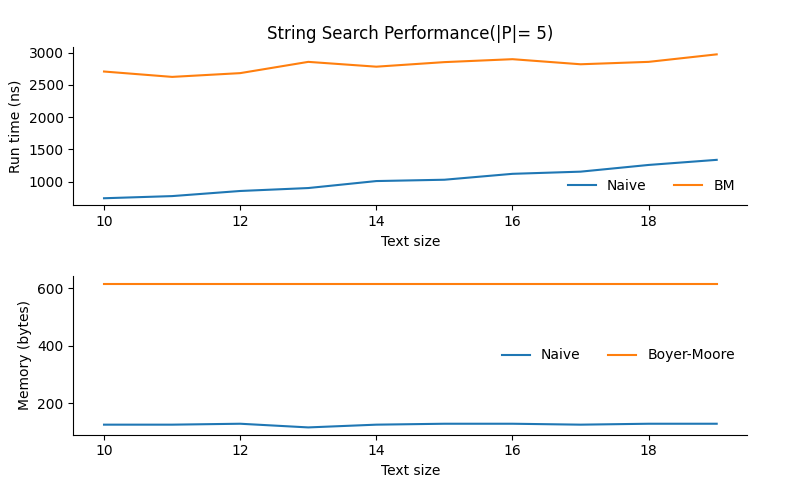
\includegraphics[width=0.75\textwidth]{time_mem/r1.png}
    \caption{Empirical runtime and memory usage of string search algorithms with $10$ rounds with pattern size $5$ and text sizes ranging from $10$ to $20$ characters with a step of $1$}
    \label{timeandmemr1}
\end{figure}

\begin{figure}[H] \centering
    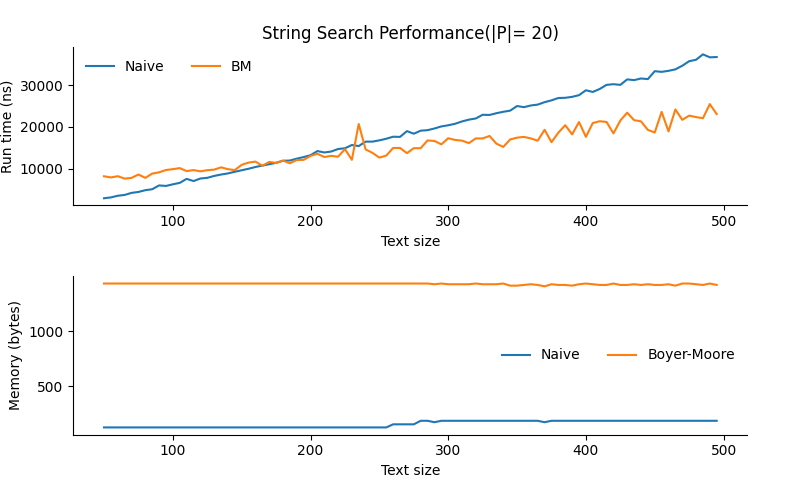
\includegraphics[width=0.75\textwidth]{time_mem/r2.png}
    \caption{Empirical runtime and memory usage of string search algorithms with $10$ rounds with pattern size $5$ and text sizes ranging from $10$ to $20$ characters with a step of $1$}
    \label{timeandmemr2}
\end{figure}

\begin{figure}[H] \centering
    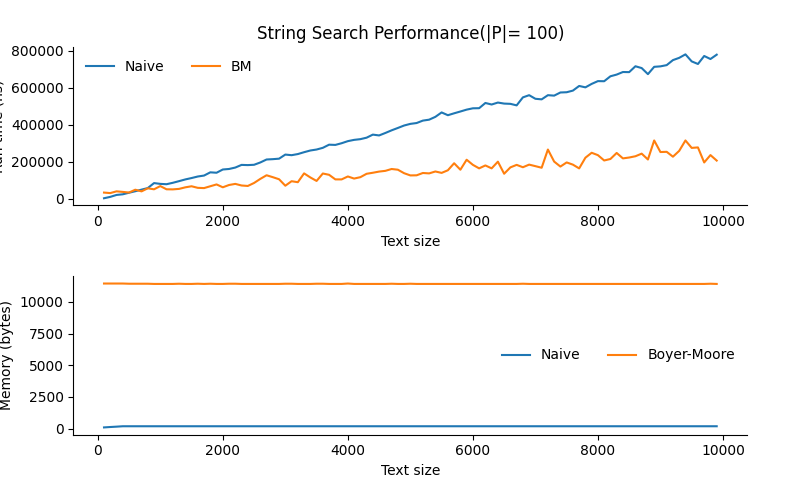
\includegraphics[width=0.75\textwidth]{time_mem/r3.png}
    \caption{Empirical runtime and memory usage of string search algorithms with $10$ rounds with pattern size $5$ and text sizes ranging from $10$ to $20$ characters with a step of $1$}
    \label{timeandmemr3}
\end{figure}

\begin{figure}[H] \centering
    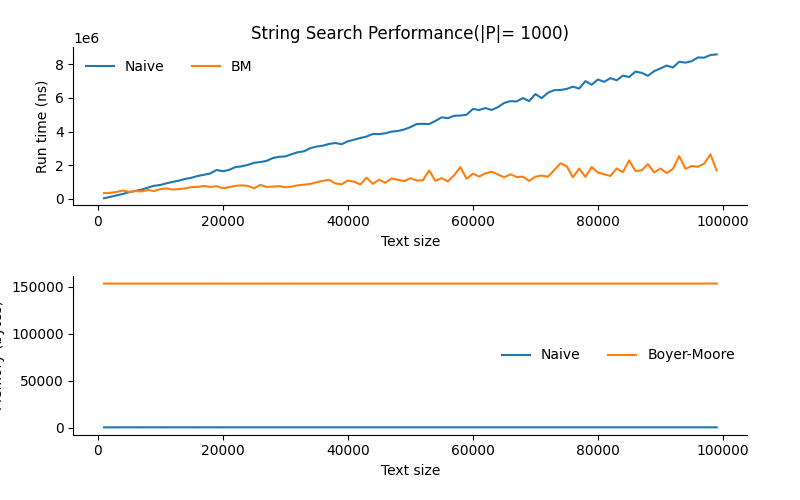
\includegraphics[width=0.75\textwidth]{time_mem/r4.png}
    \caption{Empirical runtime and memory usage of string search algorithms with $10$ rounds with pattern size $5$ and text sizes ranging from $10$ to $20$ characters with a step of $1$}
    \label{timeandmemr4}
\end{figure}

As shown in Figure \ref{timeandmemr1}, when the text size is small, and the pattern is relatively large compared to the text size, Boyer-Moore actually performs worse than the Naive search algorithm. This is likely because of the increased cost of pre-processing the data to create look-up tables. These costs are not rewarded as the search is so small and fast. Quickly, however, Boyer-Moore becomes incredibly fast compared to the Naive algorithm. In Figure \ref{timeandmemr2}, we can see at about $|T| = 225$, Boyer-Moore becomes a quicker algorithm. As $|P|$ and $|T|$ increase, so does the seperation between Boyer-Moore and the Naive algorithms' runtimes. Both algorithms' runtimes increase linearly with respect to the text size, but Boyer-Moore increases with a much smaller slope. In Figure \ref{timeandmemr4}, the slope of Boyer-Moore's runtime looks almost $0$ when compared to the massive slop of the Naive algorithm. 

The memory usage of Boyer-Moore is massive compared to that of the Naive algorithm. The Naive algorithm uses constant memory, as the text size increases, and consumes almost no Bytes. Although the memory usage of Boyer-Moore may look constant in the Figures, by analyzing the scale of the y-axis, it can clearly be seen that the memory usage increase with respect to the Pattern size. This is because storing the Good Suffix Table increases linearly with respect to $|P|$, not w.r.t $|T|$ The Bad Character Table uses a constant amount of memory in this case, defined by our alphabet. 


\subsection{Number of Shifts}
The number of shifts can be defined by the number of times the pattern moves to a new location to be compared character by character with the text. As expected, Boyer-Moore requires far fewer shifts. 

\begin{figure}[H] \centering
    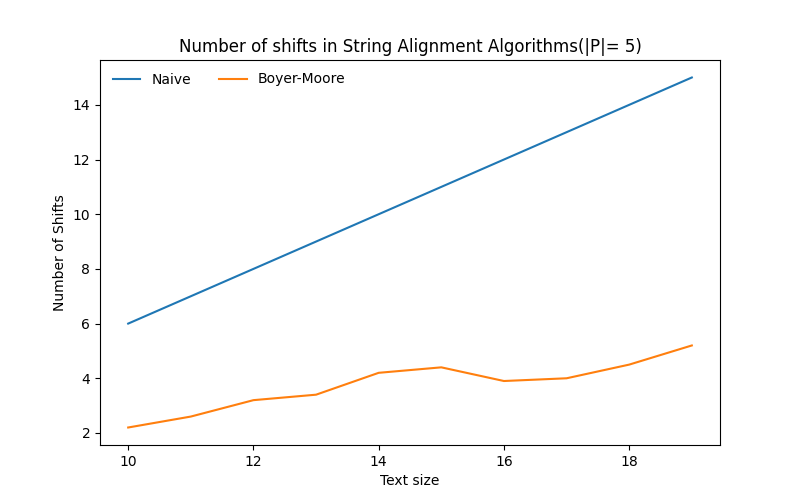
\includegraphics[width=0.75\textwidth]{shifts/r1.png}
    \caption{Empirical number of shifts of string search algorithms with $10$ rounds with pattern size $5$ and text sizes ranging from $10$ to $20$ characters with a step of $1$}
    \label{shiftsr1}
\end{figure}

\begin{figure}[H] \centering
    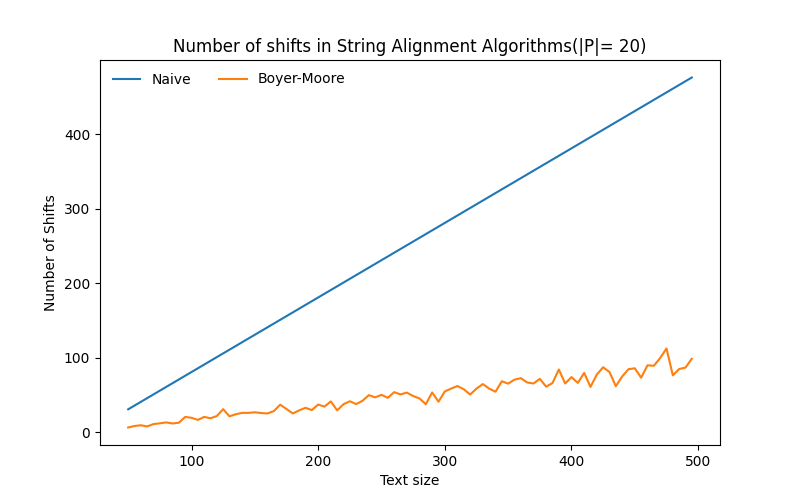
\includegraphics[width=0.75\textwidth]{shifts/r2.png}
    \caption{Empirical number of shifts of string search algorithms with $10$ rounds with pattern size $5$ and text sizes ranging from $10$ to $20$ characters with a step of $1$}
    \label{shiftsr2}
\end{figure}

\begin{figure}[H] \centering
    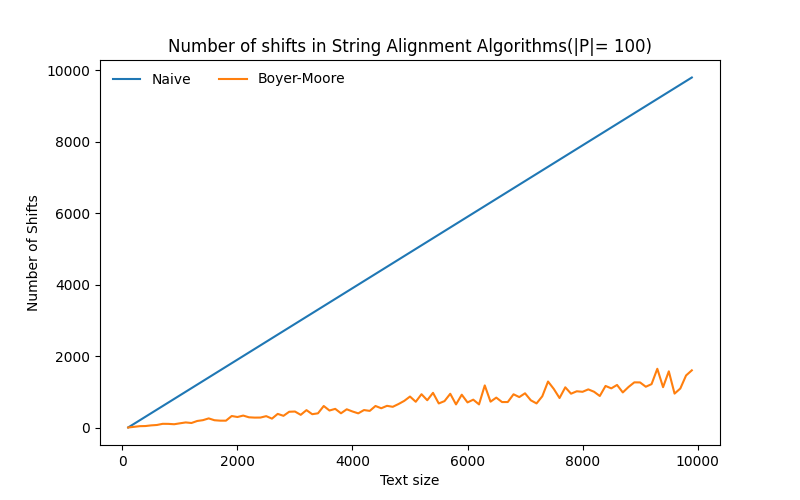
\includegraphics[width=0.75\textwidth]{shifts/r3.png}
    \caption{Empirical number of shifts of string search algorithms with $10$ rounds with pattern size $5$ and text sizes ranging from $10$ to $20$ characters with a step of $1$}
    \label{shiftsr3}
\end{figure}


\begin{figure}[H] \centering
    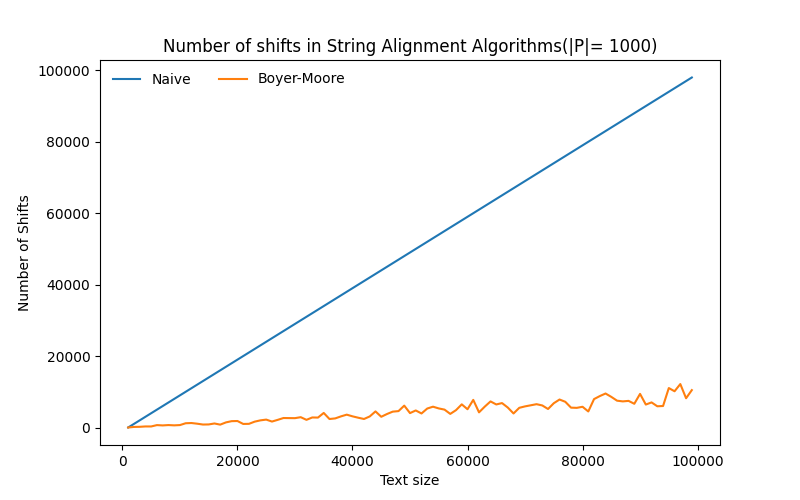
\includegraphics[width=0.75\textwidth]{shifts/r4.png}
    \caption{Empirical number of shifts of string search algorithms with $10$ rounds with pattern size $5$ and text sizes ranging from $10$ to $20$ characters with a step of $1$}
    \label{shiftsr4}
\end{figure}

The number of shifts for the Naive algorithm increases at a constant linear number with respect to the text size. This is because the pattern must be shifted and be compared at every element of the text size. In contrast, Boyer-Moore requires far fewer shifts and as the text size increases, the discrepancy only becomes larger. In the smaller text sizes, this benefit is not seen in the performance because of the cost of pre-processing, but with larger text sizes, this is the reason Boyer-Moore is so much more performant. 

\section{Methods}

\subsection{Naive string search}
The naive string search algorithm was developed by Ryan Layer and works as follows: 
\begin{displayquote}
   The naive string search algorithm considers all possible alignments of the
pattern $P$ with the text $T$. Staring at the first position in $T$, the
algorithm compares $P$'s characters with the corresponding characters in $T$.
If all characters match, the algorithm records the alignment's position in $T$.
The algorithm then repeats this process for the next alignment. If any of the 
characters in $P$ do not match a corresponding character in $T$, the current
alignment breaks and then $P$ shifts down one position in $T$, and the process
repeats. This process continues until $P$ has been compared to all possible
alignments in $T$, then returns the recorded positions. 
\end{displayquote}

\subsection{Boyer-Moore string Search}

Boyer-Moore string search was implemented to locate all occurrences of the pattern $P$ in text $T$. This algorithm was implemented using techniques from Ryan Layer's course, Robert S. Boyer's \& J. Strother Moore's original paper \cite{10.1145/359842.359859}, and with inspiration from Devin Nusbaum's interactive demonstration \cite{Nusbaum}. 

My implementation of the algorithm generates a Good Suffix look-up table (GST) according to the conventions of the Good Suffix Rule (GSR), and a Bad Character look-up table (BCT) according to the conventions of the Bad Character Rule (BCR). These tables are generated based on the standard rules for the pattern, $P$, and an example can be seen below for $P$ = ACTGAC.

\begin{figure}[ht]
    \centering
    \begin{tabular}{ |c|c|c|c|c|c|c| } 
         \hline
         $0$ & $1$ & $2$ & $3$ & $4$ & $5$ & $6$\\
         \hline
         $1$ & $7$ & $6$ &$7$ & $8$ & $9$ & $10$\\
         \hline
    \end{tabular}
    \caption{Good Suffix Table}
    \label{fig:GST}
\end{figure}

\begin{figure}[ht]
    \centering
    \begin{tabular}{ |c|c|c|c|c| } 
         \hline
         A & C & T & G & *\\
         \hline
         $1$ & $0$ & $3$ &$2$ & $6$\\
         \hline
    \end{tabular}
    \caption{Bad Character Table. Note: '*' represents the wildcard character}
    \label{fig:GST}
\end{figure}

The algorithm begins by aligning the zeroth element of $P$ and $T$, and notably, beginning the search from right to left. If an mismatch is found, the $P$ indexer is reset to the furthest right element, and the $T$ indexer is shifted the maximum of the GSR and BSR. This continues until $P$ is shifted as far right as possible. A simple and partial example using the same $P$ as above and $T$ = CCACTGACACT is shown below.

\begin{align*}
    &CCA\color{black}CT\color{blue}G\color{black}ACACT \\
    &ACTGA\color{blue}{C}
\end{align*}

Because $BCT(G) = 2$ and $GST(|P| - P_i - 1) = GST(0) = 1$, $P$ is shifted by $2$ positions. 

\begin{align*}
    CC&ACTGA\color{blue}C\color{black}ACT \\
    &ACTGA\color{blue}{C}
\end{align*}

The indices will then, continue shifting left, until, in this case the match is found, and its position is recorded.

\begin{align*}
    CC&\color{green}ACTGAC\color{black}ACT \\
    &\color{green}ACTGAC
\end{align*}

Then the process continues to check for any other occurrences. Note, because the GST and BCT are in different units, the GST index is calculated to be in terms of $T$'s indexer. 

\subsection{Empirical comparison}

The memory and time performance of the Boyer-Moore algorithm and the Naive algorithm were compared with $4$ settings in an attempt to cover a wide range of string search scenarios. Additionally, the number of shifts was recorded for with the same inputs. The inputs were ran as follows:
\begin{enumerate}
    \item $10$ rounds with pattern size $5$ and text sizes ranging from $10$ to $20$ characters with a step of $1$
    \item $5$ rounds with pattern size $20$ and text sizes ranging from $50$ to $500$ characters with a step of $5$
    \item $2$ rounds with pattern size $100$ and text sizes ranging from $100$ to $10000$ characters with a step of $100$
    \item $2$ rounds with pattern size $1000$ and text sizes ranging from $1000$ to $100000$ characters with a step of $1000$
\end{enumerate}
For each text size, I ran a single search where I generated a random
string for $T$ from the alphabet ${A, C, T, G}$ and extracted a random
substring $P$ from $T$. 

\subsection{Reproducibility}
To replicate these experiments, clone the repository and then run the
following commands from the root directory of the repository.
\begin{verbatim}
$ git clone git@github.com:cu-compg-spring-2025/assignment-4-string-search-vincedbowen.git
$ cd assignment-4-string-search-vincedbowen
\end{verbatim}
\subsubsection{Run 1}
\begin{verbatim}
    $ python src/string_search.py \
    --text_range 10 20 1 \
    --pattern_size 5 \
    --rounds 10 \
    --out_file doc/time_mem/r1.png
\end{verbatim}
\begin{verbatim}
    $ python src/string_search.py \
    --text_range 10 20 1 \
    --pattern_size 5 \
    --rounds 10 \
    --num_shifts True \
    --out_file doc/shifts/r1.png
\end{verbatim}

\subsubsection{Run 2}
\begin{verbatim}
    $ python src/string_search.py \
    --text_range 50 500 5 \
    --pattern_size 20 \
    --rounds 5 \
    --out_file doc/time_mem/r2.png
\end{verbatim}
\begin{verbatim}
    $ python src/string_search.py \
    --text_range 50 500 5 \
    --pattern_size 20 \
    --rounds 5 \
    --num_shifts True \
    --out_file doc/shifts/r2.png
\end{verbatim}

\subsubsection{Run 3}
\begin{verbatim}
    $ python src/string_search.py \
    --text_range 100 10000 100 \
    --pattern_size 100 \
    --rounds 2 \
    --out_file doc/time_mem/r3.png
\end{verbatim}
\begin{verbatim}
    $ python src/string_search.py \
    --text_range 100 10000 100 \
    --pattern_size 100 \
    --rounds 2 \
    --num_shifts True \
    --out_file doc/shifts/r3.png
\end{verbatim}

\subsubsection{Run 4}
\begin{verbatim}
    $ python src/string_search.py \
    --text_range 1000 100000 1000 \
    --pattern_size 1000 \
    --rounds 2 \
    --out_file doc/time_mem/r4.png
\end{verbatim}
\begin{verbatim}
    $ python src/string_search.py \
    --text_range 1000 100000 1000 \
    --pattern_size 1000 \
    --rounds 2 \
    --num_shifts True \
    --out_file doc/shifts/r4.png
\end{verbatim}


\bibliography{references}{}
\bibliographystyle{plain}
\end{document}
